\documentclass[report.tex]{subfiles}

\externaldocument{report}

\begin{document}

\section{原理}

\wfig{all2}に今回作ったAMラジオの全体図を示す。
今回作ったAMラジオは、ラジオ回路と増幅回路からなる。
ラジオ回路は、電波から音声信号を取り出す回路である。
増幅回路は、取り出した音声信号を増幅する回路である。

\begin{figure}[H]
	\centering
	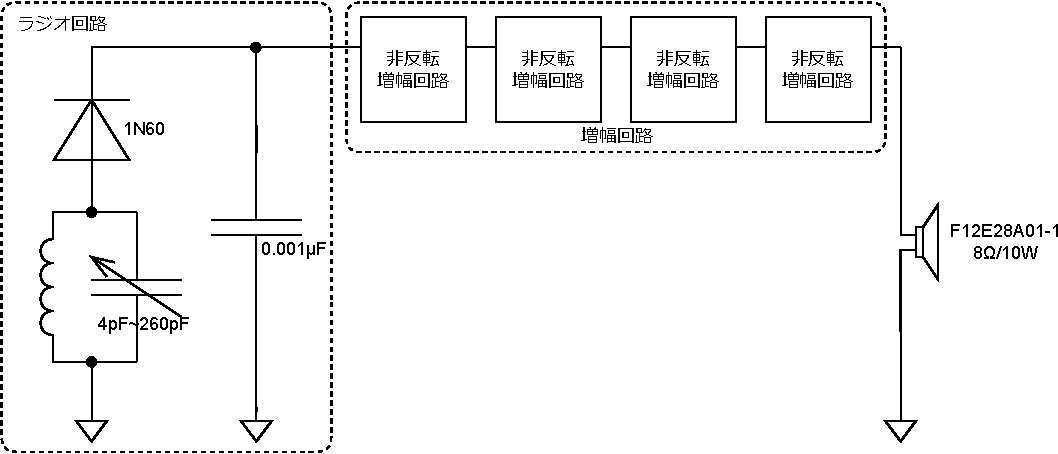
\includegraphics[width=14cm]{fig/all2.pdf}
	\caption{全体}
	\label{fig:all2}
\end{figure}

\subsection{ラジオ回路}

\wfig{radio-circuit}にラジオ回路を示す。
ラジオ回路は、電波を受信するループアンテナ、受信した電波から取り出したい周波数を選択する同調回路、受信した電波から音声周波数を取り出す検波回路からなる。

\begin{figure}[H]
	\centering
	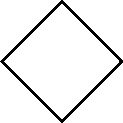
\includegraphics[width=8cm]{fig/radio.pdf}
	\caption{ラジオ回路}
	\label{fig:radio-circuit}
\end{figure}

\subsubsection{ループアンテナ}

\wfig{radio-circuit}で用いられているループアンテナは、巻き線をループ状に巻いたものである。
ループアンテナは、電波の磁界成分で誘導起電力を引き起こし、電流が流れる。
この電流を誘導電流という。
電波の磁界成分で誘導起電力を引き起こすのは、以下より求めることができる。
ここで、\(B[\rm{T}]\)は磁束密度、\(\mu[\rm{H/m}]\)は透磁率、\(H[\rm{A/m}]\)は磁界の強さ、\(S[\rm{m^2}]\)はループアンテナの面積、\(N[\rm{turn}]\)はループアンテナの巻数、\(\Phi[\rm{Wb}]\)は磁束である。
式より、磁界の強さの変化によって、誘導起電力が発生し、透磁率、巻き数、ループアンテナの面積に比例していることがわかる。

\begin{align}
	B = \mu H               \\
	\Phi = B S              \\ % TODO 電磁気の本
	V = -N \frac{d\Phi}{dt} \\
	V = -N S \mu \frac{dH}{dt}
\end{align}

\subsubsection{同調回路}

同調回路は、様々な周波数の電波から、特定の周波数の電波を取り出す回路である。

\begin{align}
	Z & = \frac{j \omega L \times \frac{1}{j \omega C}}{j \omega L + \frac{1}{j \omega C}} \\
	  & = \frac{j \omega L}{1 - \omega^2 LC}                                               \\
\end{align}

ここで、$\omega^2 LC = 1$と仮定すると、インピーダンス\(Z\)は無限大となる。
この時の周波数\(f\)は以下のようにして決定することが出きる。

\begin{align}
	\omega^2 LC & = 1                                              \\
	\omega      & = \frac{1}{\sqrt{LC}}                            \\
	f           & = \frac{1}{2 \pi \sqrt{LC}} \label{eq:resonance}
\end{align}

\wfig{tuning-circuit}では、同調回路のキャパシタンス部分に可変コンデンサ(バリアブルコンデンサ)を用いている。
そのため、可変コンデンサの容量を変えることで、受信したい周波数を変えることができる。
AMラジオでは、\wtab{zuishin}のような受信局(東京)がある。

\begin{table}[h]
	\centering
	\caption{AMラジオの受信局(東京)}
	\label{tab:zyushin}
	\begin{tabular}{ccccc} \hline
		放送局    & 周波数[kHz] & 送信出力[kW] & 学校までの距離[km] & 受信できる周波数[kHz]           \\ \hline
		NHK第1  & 594      & 300      & 40          & 40 \(\sim\) 3949.80     \\
		NHK第2  & 693      & 500      & 40          & 40 \(\sim\) 2388.26     \\
		AFN    & 810      & 50       & 45          & 600.69 \(\sim\) 4842.93 \\
		TBSラジオ & 954      & 100      & 60          & 346.23 \(\sim\) 2790.26 \\
		ニッポン放送 & 1134     & 100      & 32          & 155.69 \(\sim\) 1255.93 \\
		文化放送   & 1242     & 100      & 18          & 170.69 \(\sim\) 1377.93 \\
		ラジオ日本  & 1422     & 50       & 7           & 136.23 \(\sim\) 1099.26 \\ \hline
	\end{tabular}
\end{table}

\subsubsection{検波回路}

検波回路とは、電波から受け取った信号から音声信号を取り出す回路である。
今回作ったラジオは、振幅変調波(AM)を受信する回路である。
振幅変調波は、\wfig{5V}のような搬送波と、\wfig{3V}のような信号波を用いて、\wfig{wave}のような電波として送信される。
ここで、搬送波\(v_c\)の振幅を\(V_{cm}\)、周波数を\(f_c\)、信号波\(v_s\)の振幅を\(V_{sm}\)、周波数を\(f_s\)とすると、それぞれ次式のように表すことができる。

\begin{align}
	v_c = V_{cm} \sin(2 \pi f_c t) \\
	v_s = V_{sm} \sin(2 \pi f_s t) \\
\end{align}

\begin{figure}[H]
	\begin{minipage}[b]{0.5\columnwidth}
		\centering
		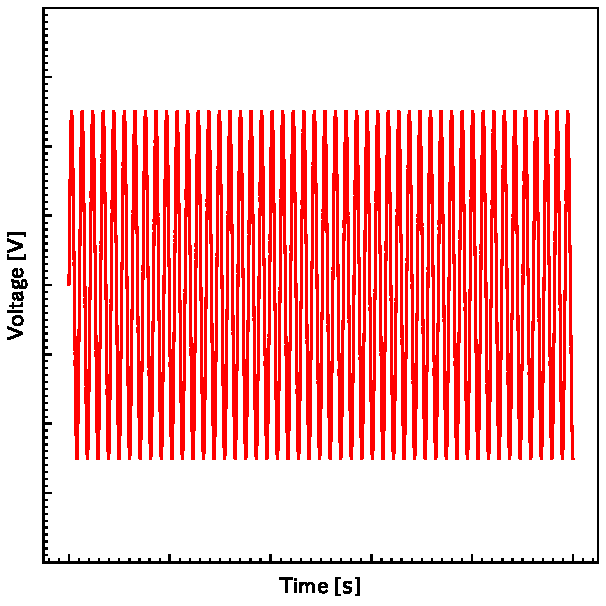
\includegraphics[width=8cm]{fig/5V.pdf}
		\caption{搬送波}
		\label{fig:5V}
	\end{minipage}
	\begin{minipage}[b]{0.5\columnwidth}
		\centering
		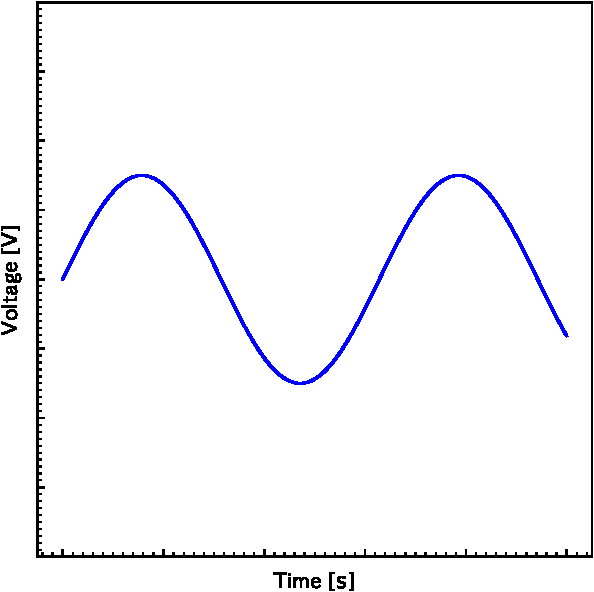
\includegraphics[width=8cm]{fig/3V.pdf}
		\caption{信号波}
		\label{fig:3V}
	\end{minipage}
\end{figure}

振幅変調波\(v_o\)は、次式で表すことができ、\wfig{wave}のような波形になる。

\begin{align}
	v_o = (V_{cm} + V_{sm} \sin(2 \pi f_s t)) \sin(2 \pi f_c t)
\end{align}

\begin{figure}[H]
	\centering
	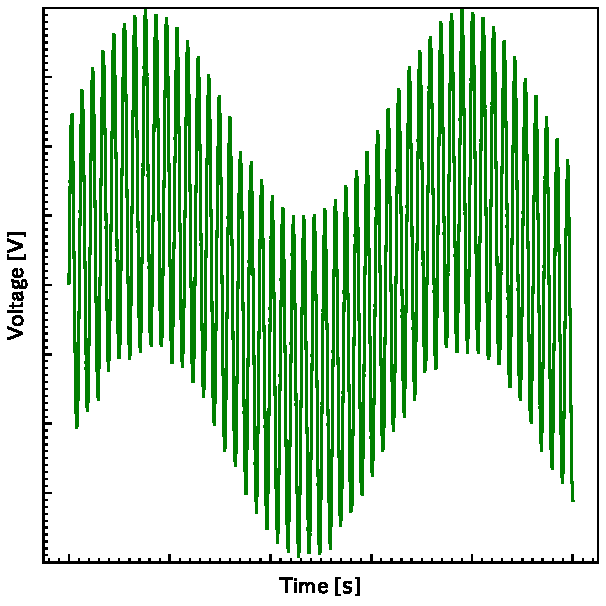
\includegraphics[width=8cm]{fig/Wave.pdf}
	\caption{電波から受信された信号(振幅変調波)}
	\label{fig:wave}
\end{figure}

検波回路ではまず、ゲルマニウムダイオードを用いて、\wfig{diode}のような波形にする。
ダイオードには、順方向特性(逆方向に電圧がかからない)があるため、電圧がマイナスになっている部分はカットされる。

\begin{figure}[H]
	\centering
	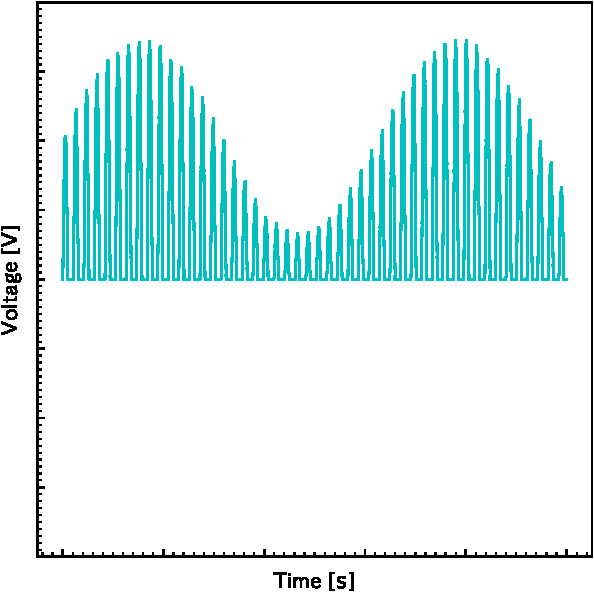
\includegraphics[width=8cm]{fig/diode.pdf}
	\caption{ダイオードで逆方向電圧を取り除いた信号}
	\label{fig:diode}
\end{figure}

また、0.001\(\upmu\)Fのコンデンサを用いて、搬送波部分を取り除く。
キャパシタンスは、搬送波のような高い周波数に対しては、インピーダンスが小さくなる。
逆に、信号波のような低い周波数に対しては、インピーダンスが大きくなる。
そのため、\wfig{capa}のように搬送波が取り除かれて、信号波のみが残る。

\begin{figure}[H]
	\centering
	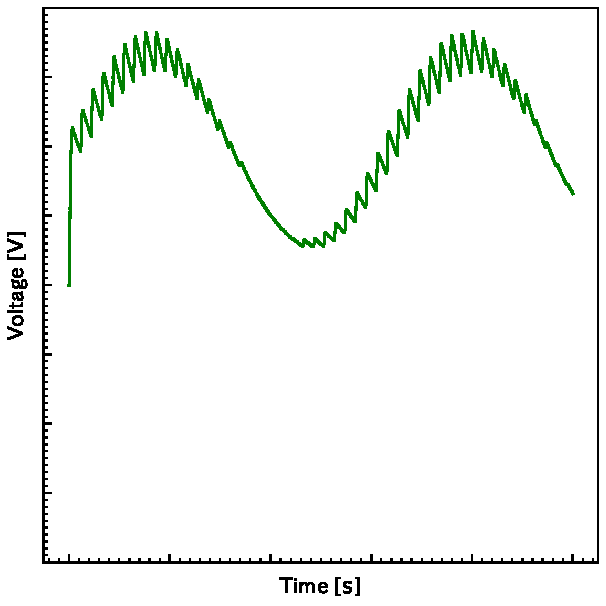
\includegraphics[width=8cm]{fig/capa.pdf}
	\caption{キャパシタンスで搬送波部分を取り除いた信号}
	\label{fig:capa}
\end{figure}

\subsection{増幅回路}

\wfig{amplifier-circuit}に増幅回路を示す。
\wfig{amplifier-circuit}は、\wfig{amplifier-circuit2}のような非反転増幅回路を用いて設計されている。
オペアンプ
非反転増幅回路の増幅度\(A_{vf}\)は、次のように表される。

\begin{align}
	A_{vf} = 1 + \frac{R_2}{R_1}
\end{align}

\begin{figure}[H]
	\centering
	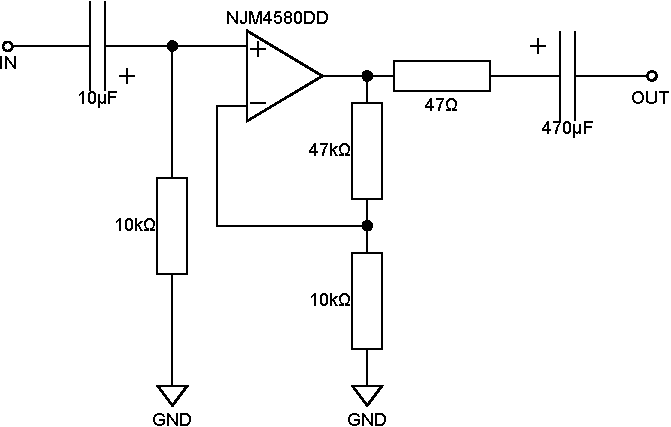
\includegraphics[width=15cm]{fig/amp.pdf}
	\caption{増幅回路}
	\label{fig:amplifier-circuit}
\end{figure}

\begin{figure}[H]
	\centering
	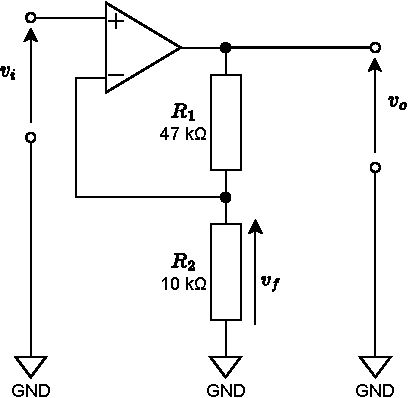
\includegraphics[width=8cm]{fig/amp2.pdf}
	\caption{非反転増幅回路}
	\label{fig:amplifier-circuit2}
\end{figure}

\subsection{可変抵抗(ボリューム)}

可変抵抗には、主にAカーブとBカーブとCカーブなどの種類がある。
\wfig{cabe}にそれぞれのカーブの特性を示す。
Aカーブは、回転角度に対して、抵抗値が指数関数的に上昇する。
Bカーブは、回転角度に対して、抵抗値が比例的に上昇する。
Cカーブは、回転角度に対して、抵抗値が対数関数的に上昇する。
人間の耳は、オーディオの出力信号に対して比例的に感じることはなく、その対数に比例して感じる(小さい音に敏感に反応する)。
そのため、オーディオの音量調節には、Aカーブの可変抵抗を用いることが多い。

\begin{figure}[H]
	\centering
	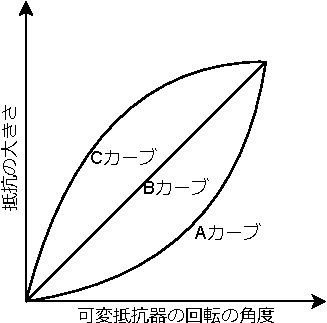
\includegraphics[width=8cm]{fig/cabe.pdf}
	\caption{可変抵抗のカーブ}
	\label{fig:cabe}
\end{figure}

\end{document}
